\section*{Лекция 3 (03.03.2022)}

$f \in C^2[a, b]$ \,\,\, $\theta = \{ x_0 = a, x_1, ... , x_n = b\}$

\[
    \abs{\int_a^b {f} dx - \sum_{j = 1} ^ n \frac{f(x_j) + f(x_{j - 1})}{2}} \leqslant \frac{\abs{\theta} ^ 2}{8} \int_a^b \abs{f''}, \text{ где } \abs{\theta} = \max{\abs{x_j - x_{j - 1}}} \text{ --- мелкость(ранг) разбиения}  
\]

\begin{proof}
    \begin{enumerate}
        \item Разбиения в этой теореме не нужно. Достаточно доказать для отрезка, где $x_0 = a, x_1 = b$.
        
        \[
            \int_a^b \abs{f''} = \sum \int_{x_{j - 1}}^{x_j}
        \]

        \[
            \int_a^b {f} dx = \sum \int_{x_{j - 1}}^{x_j}
        \]

        Сводим к неравенству:

        \[
            \abs{\int_a^b f - \frac{f(a) + f(b)}{2} \cdot (b - a)} \leqslant \frac{(b - a) ^ 2}{8} \cdot \int_a^b \abs{f''}
        \]

        \item Рассмотрим разностное отношение функциий. Для этого введем $g$ - линейная функция, такая что $g(a) = f(a), g(b) = f(b)$.
        
        \[
            \Rightarrow \int_a^b f - \frac{f(a) + f(b)}{2} \cdot (b - a) = \int_a^b {f - g}, \text{ но $g'' = 0$} \Rightarrow
        \]

        \[
            \int_a^b \abs{f''} = \int_a^b \abs{f'' - g''} = \int_a^b \abs{(f - g)''}
        \]

        \item Свели утверждение к 
        
        \[
            \abs{\int_a^b f} \leqslant \frac{(b - a) ^ 2}{8} \int_a^b \abs{f''}, f \in C^2[a, b], f(a) = f(b) = 0, \text{ где $f$ на самом деле $f - g$}
        \]

        \[
            \int_a^b f(x) dx = \int_a^b f(x) d (x - \alpha) = f(x) (x - \alpha) \bigg |_a^b - \int_a^b (x - \alpha) f'(x) dx = 0 - \int_a^b (x - \alpha) f'(x) dx =
        \]

        \[
            -\int_a^b f'(x) d \left(\frac{x ^ 2}{2} - \alpha x + \beta \right) = - f'(x) \left( \frac{x ^ 2}{2} - \alpha x + \beta \right) \bigg |_a^b + \int_a^b f''(x) \left(\frac{x ^ 2}{2} - \alpha x + \beta \right) dx \ceq
        \]

        \[
            \alpha, \beta : \frac{(x - a)(x - b)}{2} = \frac{x ^ 2}{2} - \alpha x + \beta 
        \]

        \[
            \ceq \int_a^b f''(x) \frac{(x - a)(x - b)}{2} dx
        \]

        \[
            \abs{\frac{(x - a)(x - b)}{2}} \leqslant \left( \frac{b - a}{2} \right) ^ 2 \cdot \frac{1}{2} = \frac{(b - a) ^ 2}{8}
        \]

        \[
            \abs{\int_a^b f } \leqslant \frac{(b - a)^2}{8} \int_a^b \abs{f''}
        \]
    \end{enumerate}
\end{proof}


\follow \,(для равномерного дробления)

Если $x_0 = a, x_1 = a + \frac{b - a}{n}, ... x_n = b$, то

\[
    \abs{\int_a^b f(x) dx - \sum_{j = 1} ^ n \frac{f(x_j) - f(x_{j - 1})}{2} \cdot \frac{b - a}{n}}  \leqslant \frac{(b - a) ^ 2}{8 \cdot n^2} \int_a^b \abs{f''}
\]

\quad 

\begin{namedtheorem}{формула Эйлера-Маклорена}
    \[
        f \in C^2[m, n], \, m < n, \, f(m) + f(m + 1) + ... + f(n) = \, ?
    \]
\end{namedtheorem} 

\begin{proof}
    \[
        \int_m^n f dx - \sum_{j = m + 1}^n \frac{f(j) + f(j - 1)}{2}  = \int_m^n f''(x) \frac{\{x \} (\{x \} - 1)}{2} dx \text{(для подробностей 29 минута \href{https://drive.google.com/file/d/1PE4c82vhdcEngDkpNyRiATNBhnSxje4S/view}{записи}} ) 
    \]

    Все кроме крайних ($f(m) $ и $f(n)$) по 2 раза в 

    \[
        \sum_{i = m + 1}^n \frac{f(i) + f(i - 1)}{2}
    \] 

    Поэтому 

    \[
        f(m) + ... + f(n) = \frac{f(m) + f(n)}{2} + \int_m^n f dx + \int_m^n f''(x) \frac{\{x\}(1 - \{x \})}{2} dx
    \]
\end{proof}

\begin{examples}
    \begin{enumerate}
        \item \[
        H_n = 1 + \frac{1}{2} + ... + \frac{1}{n}, f(x) = \frac{1}{x}
    \]

    \[
        H_n = \frac{1 + \frac{1}{n}}{2} + \underbrace{\int_1^n \frac{dx}{x}}_{= \ln n} + \underbrace{\int_1^n \frac{2}{x ^ 3} \cdot \frac{\{ x \}(1 - \{ x\})}{2}}_{= I_n} dx
    \]

    \[
        I_n \leqslant \int_1^n \frac{dx}{x ^ 3} = - \frac{1}{2 x ^ 2} \bigg|_1^n = \frac{1}{2} - \frac{1}{2 n ^ 2}
    \]

    \[
        H_n = \ln n + \frac{1}{2} + \frac{1}{2n} + I_n = \ln n + \delta + o(1) 
    \]

    $I_n $ -- возрастает и ограничена, где $\delta$ - нек. конст. Эйлера (про нее неизвестного ничего, кроме миллиона знаков после запятой :)
\newpage
    \item (формула Стирлинга) 
    $n! \sim \sqrt{2 \pi n} \left( \frac{n}{e} \right) ^ n, n \to \infty$ 
    
    $\but$ не следует думать, что факториал равен этой штуке, это означает только то, что отношение стремится к единице

    \[
        n! = \sqrt{2 \pi n}\left(\frac{n}{e} \right) ^ n (1 + \frac{1}{12n} + o\left(\frac{1}{n} \right))
    \]

    $\but$ Ошибка на $(n - 1)!$

    \[
        \ln n! = \ln 1 + ... + \ln n = \frac{\ln 1 + \ln n}{2} + \int_1^n \ln x dx + \underbrace{\int_1^n (\ln x)'' \frac{\{ x\}(1 - \{ x \})}{2} dx}_{\int_1^n - \frac{1}{x ^ 2} ... = I_n} = 
    \]

    \[
        = n \ln n - n + 1 + \frac{\ln n}{2} + I_n  \ceq
    \]
    
    \[
        \abs{I_n} \leqslant \int_1^n \frac{1}{x ^ 2} = 1 - \frac{1}{n}
    \]

    \[
        \ceq n \ln n - n + \frac{\ln n}{2} + \ln const + o(1), \text{ т.к. } I_n = O(1)
    \]

    \[
        \hence n! \sim \frac{n ^ n}{e ^ n} \sqrt{n} \cdot c
    \]


    Применим формулу Валисса
    \[
        C_{2n}^{n} = \frac{(2n)!}{n! n!} \sim \frac{\left( \frac{2n}{e} \right) ^ {2n} \sqrt{2n} \cdot c }{\left( \left( \frac{n}{e} \right) ^ n \sqrt{n} \cdot c \right) ^ 2} = \frac{1}{c} \cdot 4 ^ n \cdot \frac{1}{\sqrt{n}} \cdot \sqrt{2} \hence c = \sqrt{2 \pi}
    \]
    \end{enumerate}
\end{examples}

\newpage

\section{Несобственный интеграл}

\begin{motivation}
    \[
        \int_0^\pi \frac{dx}{2 + \cos x} = \left[ t = \tg \frac{x}{2} \right] = \int_0^{\tg \frac{\pi}{2} = +\infty} ... \,\, dt 
    \]

    Как с таким бороться?

    Пишем неопределенный интеграл, считаем его и подставляем.
\end{motivation}

\begin{definition}
    $f \in C[a, b],  b \in \R \cup \{ + \infty \}$

    $\underbrace{\int_a^{\to b} f dx}_{\text{Несобственный интеграл}} = \lim_{B \to b-} \int_a^B f dx$ --- частичный интеграл
\\
\begin{itemize}
    \item сх-ся $\Longleftrightarrow \exists \lim$ --- конечный
    \item расх-ся $\Longleftrightarrow \nexists \lim$
\end{itemize}
    
\end{definition}


2 ситуации, в которых это бывает полезно: \\\\\\

\tikzset{every picture/.style={line width=0.75pt}} %set default line width to 0.75pt        

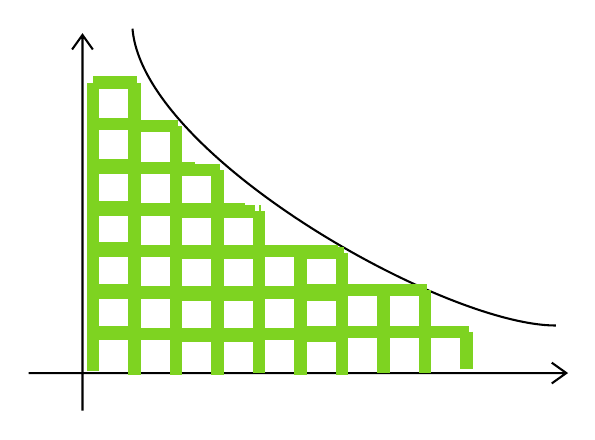
\begin{tikzpicture}[x=0.75pt,y=0.75pt,yscale=-1,xscale=1]
%uncomment if require: \path (0,300); %set diagram left start at 0, and has height of 300

%Shape: Axis 2D [id:dp10588915447714264] 
\draw  (131,237.9) -- (390,237.9)(156.9,75) -- (156.9,256) (383,232.9) -- (390,237.9) -- (383,242.9) (151.9,82) -- (156.9,75) -- (161.9,82)  ;
%Curve Lines [id:da2919012249645151] 
\draw    (181,72) .. controls (186,133) and (331,215) .. (385,215) ;
%Shape: Grid [id:dp2527585760344795] 
\draw  [draw opacity=0][line width=4.5]  (162,139) -- (211,139) -- (211,214) -- (162,214) -- cycle ; \draw  [color={rgb, 255:red, 126; green, 211; blue, 33 }  ,draw opacity=1 ][line width=4.5]  (162,139) -- (162,214)(182,139) -- (182,214)(202,139) -- (202,214) ; \draw  [color={rgb, 255:red, 126; green, 211; blue, 33 }  ,draw opacity=1 ][line width=4.5]  (162,139) -- (211,139)(162,159) -- (211,159)(162,179) -- (211,179)(162,199) -- (211,199) ; \draw  [color={rgb, 255:red, 126; green, 211; blue, 33 }  ,draw opacity=1 ][line width=4.5]   ;
%Shape: Grid [id:dp4396197006457828] 
\draw  [draw opacity=0][line width=4.5]  (162,159) -- (215,159) -- (215,237) -- (162,237) -- cycle ; \draw  [color={rgb, 255:red, 126; green, 211; blue, 33 }  ,draw opacity=1 ][line width=4.5]  (162,159) -- (162,237)(182,159) -- (182,237)(202,159) -- (202,237) ; \draw  [color={rgb, 255:red, 126; green, 211; blue, 33 }  ,draw opacity=1 ][line width=4.5]  (162,159) -- (215,159)(162,179) -- (215,179)(162,199) -- (215,199)(162,219) -- (215,219) ; \draw  [color={rgb, 255:red, 126; green, 211; blue, 33 }  ,draw opacity=1 ][line width=4.5]   ;
%Shape: Grid [id:dp2561618352819087] 
\draw  [draw opacity=0][line width=4.5]  (182,159) -- (235,159) -- (235,237) -- (182,237) -- cycle ; \draw  [color={rgb, 255:red, 126; green, 211; blue, 33 }  ,draw opacity=1 ][line width=4.5]  (182,159) -- (182,237)(202,159) -- (202,237)(222,159) -- (222,237) ; \draw  [color={rgb, 255:red, 126; green, 211; blue, 33 }  ,draw opacity=1 ][line width=4.5]  (182,159) -- (235,159)(182,179) -- (235,179)(182,199) -- (235,199)(182,219) -- (235,219) ; \draw  [color={rgb, 255:red, 126; green, 211; blue, 33 }  ,draw opacity=1 ][line width=4.5]   ;
%Shape: Grid [id:dp032426188030667324] 
\draw  [draw opacity=0][line width=4.5]  (182,159) -- (235,159) -- (235,237) -- (182,237) -- cycle ; \draw  [color={rgb, 255:red, 126; green, 211; blue, 33 }  ,draw opacity=1 ][line width=4.5]  (182,159) -- (182,237)(202,159) -- (202,237)(222,159) -- (222,237) ; \draw  [color={rgb, 255:red, 126; green, 211; blue, 33 }  ,draw opacity=1 ][line width=4.5]  (182,159) -- (235,159)(182,179) -- (235,179)(182,199) -- (235,199)(182,219) -- (235,219) ; \draw  [color={rgb, 255:red, 126; green, 211; blue, 33 }  ,draw opacity=1 ][line width=4.5]   ;
%Shape: Grid [id:dp15673758254887082] 
\draw  [draw opacity=0][line width=4.5]  (222,179) -- (267,179) -- (267,237) -- (222,237) -- cycle ; \draw  [color={rgb, 255:red, 126; green, 211; blue, 33 }  ,draw opacity=1 ][line width=4.5]  (222,179) -- (222,237)(242,179) -- (242,237)(262,179) -- (262,237) ; \draw  [color={rgb, 255:red, 126; green, 211; blue, 33 }  ,draw opacity=1 ][line width=4.5]  (222,179) -- (267,179)(222,199) -- (267,199)(222,219) -- (267,219) ; \draw  [color={rgb, 255:red, 126; green, 211; blue, 33 }  ,draw opacity=1 ][line width=4.5]   ;
%Shape: Grid [id:dp2299385849156933] 
\draw  [draw opacity=0][line width=4.5]  (202,160) -- (240,160) -- (240,237) -- (202,237) -- cycle ; \draw  [color={rgb, 255:red, 126; green, 211; blue, 33 }  ,draw opacity=1 ][line width=4.5]  (202,160) -- (202,237)(222,160) -- (222,237) ; \draw  [color={rgb, 255:red, 126; green, 211; blue, 33 }  ,draw opacity=1 ][line width=4.5]  (202,160) -- (240,160)(202,180) -- (240,180)(202,200) -- (240,200)(202,220) -- (240,220) ; \draw  [color={rgb, 255:red, 126; green, 211; blue, 33 }  ,draw opacity=1 ][line width=4.5]   ;
%Shape: Grid [id:dp9837712632464429] 
\draw  [draw opacity=0][line width=4.5]  (262,198) -- (292,198) -- (292,237) -- (262,237) -- cycle ; \draw  [color={rgb, 255:red, 126; green, 211; blue, 33 }  ,draw opacity=1 ][line width=4.5]  (262,198) -- (262,237)(282,198) -- (282,237) ; \draw  [color={rgb, 255:red, 126; green, 211; blue, 33 }  ,draw opacity=1 ][line width=4.5]  (262,198) -- (292,198)(262,218) -- (292,218) ; \draw  [color={rgb, 255:red, 126; green, 211; blue, 33 }  ,draw opacity=1 ][line width=4.5]   ;
%Shape: Grid [id:dp6226580372622806] 
\draw  [draw opacity=0][line width=4.5]  (302,218) -- (343,218) -- (343,236) -- (302,236) -- cycle ; \draw  [color={rgb, 255:red, 126; green, 211; blue, 33 }  ,draw opacity=1 ][line width=4.5]  (302,218) -- (302,236)(322,218) -- (322,236)(342,218) -- (342,236) ; \draw  [color={rgb, 255:red, 126; green, 211; blue, 33 }  ,draw opacity=1 ][line width=4.5]  (302,218) -- (343,218) ; \draw  [color={rgb, 255:red, 126; green, 211; blue, 33 }  ,draw opacity=1 ][line width=4.5]   ;
%Shape: Grid [id:dp27910164052736075] 
\draw  [draw opacity=0][line width=4.5]  (162,98) -- (183,98) -- (183,237) -- (162,237) -- cycle ; \draw  [color={rgb, 255:red, 126; green, 211; blue, 33 }  ,draw opacity=1 ][line width=4.5]  (162,98) -- (162,237)(182,98) -- (182,237) ; \draw  [color={rgb, 255:red, 126; green, 211; blue, 33 }  ,draw opacity=1 ][line width=4.5]  (162,98) -- (183,98)(162,118) -- (183,118)(162,138) -- (183,138)(162,158) -- (183,158)(162,178) -- (183,178)(162,198) -- (183,198)(162,218) -- (183,218) ; \draw  [color={rgb, 255:red, 126; green, 211; blue, 33 }  ,draw opacity=1 ][line width=4.5]   ;
%Shape: Grid [id:dp07057802687886527] 
\draw  [draw opacity=0][line width=4.5]  (182,119) -- (203,119) -- (203,239) -- (182,239) -- cycle ; \draw  [color={rgb, 255:red, 126; green, 211; blue, 33 }  ,draw opacity=1 ][line width=4.5]  (182,119) -- (182,239)(202,119) -- (202,239) ; \draw  [color={rgb, 255:red, 126; green, 211; blue, 33 }  ,draw opacity=1 ][line width=4.5]  (182,119) -- (203,119)(182,139) -- (203,139)(182,159) -- (203,159)(182,179) -- (203,179)(182,199) -- (203,199)(182,219) -- (203,219) ; \draw  [color={rgb, 255:red, 126; green, 211; blue, 33 }  ,draw opacity=1 ][line width=4.5]   ;
%Shape: Grid [id:dp8322125574901823] 
\draw  [draw opacity=0][line width=4.5]  (202,140) -- (223,140) -- (223,239) -- (202,239) -- cycle ; \draw  [color={rgb, 255:red, 126; green, 211; blue, 33 }  ,draw opacity=1 ][line width=4.5]  (202,140) -- (202,239)(222,140) -- (222,239) ; \draw  [color={rgb, 255:red, 126; green, 211; blue, 33 }  ,draw opacity=1 ][line width=4.5]  (202,140) -- (223,140)(202,160) -- (223,160)(202,180) -- (223,180)(202,200) -- (223,200)(202,220) -- (223,220) ; \draw  [color={rgb, 255:red, 126; green, 211; blue, 33 }  ,draw opacity=1 ][line width=4.5]   ;
%Shape: Grid [id:dp17766547342352357] 
\draw  [draw opacity=0][line width=4.5]  (242,160) -- (243,160) -- (243,238) -- (242,238) -- cycle ; \draw  [color={rgb, 255:red, 126; green, 211; blue, 33 }  ,draw opacity=1 ][line width=4.5]  (242,160) -- (242,238) ; \draw  [color={rgb, 255:red, 126; green, 211; blue, 33 }  ,draw opacity=1 ][line width=4.5]  (242,160) -- (243,160)(242,180) -- (243,180)(242,200) -- (243,200)(242,220) -- (243,220) ; \draw  [color={rgb, 255:red, 126; green, 211; blue, 33 }  ,draw opacity=1 ][line width=4.5]   ;
%Shape: Grid [id:dp7749771471385206] 
\draw  [draw opacity=0][line width=4.5]  (282,198) -- (315,198) -- (315,237) -- (282,237) -- cycle ; \draw  [color={rgb, 255:red, 126; green, 211; blue, 33 }  ,draw opacity=1 ][line width=4.5]  (282,198) -- (282,237)(302,198) -- (302,237) ; \draw  [color={rgb, 255:red, 126; green, 211; blue, 33 }  ,draw opacity=1 ][line width=4.5]  (282,198) -- (315,198)(282,218) -- (315,218) ; \draw  [color={rgb, 255:red, 126; green, 211; blue, 33 }  ,draw opacity=1 ][line width=4.5]   ;
%Shape: Grid [id:dp9928358645742608] 
\draw  [draw opacity=0][line width=4.5]  (262,179) -- (280,179) -- (280,236) -- (262,236) -- cycle ; \draw  [color={rgb, 255:red, 126; green, 211; blue, 33 }  ,draw opacity=1 ][line width=4.5]  (262,179) -- (262,236) ; \draw  [color={rgb, 255:red, 126; green, 211; blue, 33 }  ,draw opacity=1 ][line width=4.5]  (262,179) -- (280,179)(262,199) -- (280,199)(262,219) -- (280,219) ; \draw  [color={rgb, 255:red, 126; green, 211; blue, 33 }  ,draw opacity=1 ][line width=4.5]   ;
%Shape: Grid [id:dp34183885120601276] 
\draw  [draw opacity=0][line width=4.5]  (262,180) -- (283,180) -- (283,239) -- (262,239) -- cycle ; \draw  [color={rgb, 255:red, 126; green, 211; blue, 33 }  ,draw opacity=1 ][line width=4.5]  (262,180) -- (262,239)(282,180) -- (282,239) ; \draw  [color={rgb, 255:red, 126; green, 211; blue, 33 }  ,draw opacity=1 ][line width=4.5]  (262,180) -- (283,180)(262,200) -- (283,200)(262,220) -- (283,220) ; \draw  [color={rgb, 255:red, 126; green, 211; blue, 33 }  ,draw opacity=1 ][line width=4.5]   ;
%Shape: Grid [id:dp648164858914508] 
\draw  [draw opacity=0][line width=4.5]  (302,198) -- (323,198) -- (323,238) -- (302,238) -- cycle ; \draw  [color={rgb, 255:red, 126; green, 211; blue, 33 }  ,draw opacity=1 ][line width=4.5]  (302,198) -- (302,238)(322,198) -- (322,238) ; \draw  [color={rgb, 255:red, 126; green, 211; blue, 33 }  ,draw opacity=1 ][line width=4.5]  (302,198) -- (323,198)(302,218) -- (323,218) ; \draw  [color={rgb, 255:red, 126; green, 211; blue, 33 }  ,draw opacity=1 ][line width=4.5]   ;




\end{tikzpicture}




\tikzset{every picture/.style={line width=0.75pt}} %set default line width to 0.75pt        

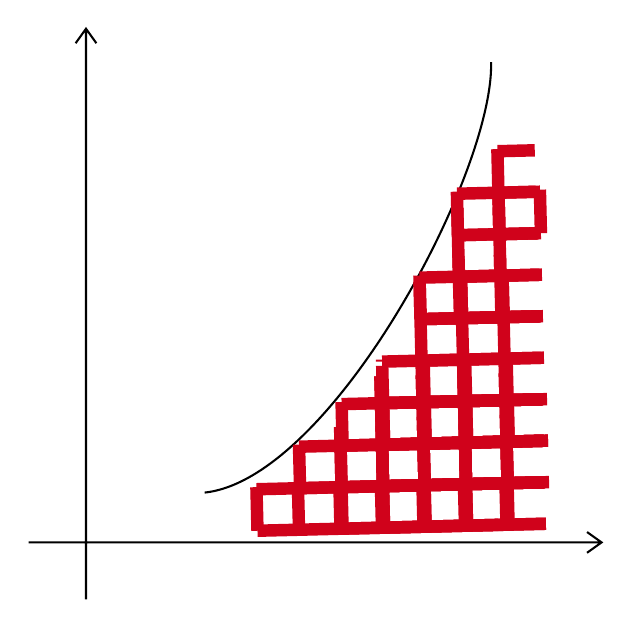
\begin{tikzpicture}[x=0.75pt,y=0.75pt,yscale=-1,xscale=1]
%uncomment if require: \path (0,300); %set diagram left start at 0, and has height of 300

%Curve Lines [id:da2919012249645151] 
\draw    (192.77,250.49) .. controls (253.63,244.01) and (332.09,97.06) .. (330.78,43.08) ;
%Shape: Grid [id:dp2527585760344795] 
\draw  [draw opacity=0][line width=4.5]  (259.21,267.88) -- (258.02,218.89) -- (333,217.07) -- (334.19,266.06) -- cycle ; \draw  [color={rgb, 255:red, 208; green, 2; blue, 27 }  ,draw opacity=1 ][line width=4.5]  (259.21,267.88) -- (334.19,266.06)(258.72,247.89) -- (333.7,246.07)(258.24,227.89) -- (333.22,226.07) ; \draw  [color={rgb, 255:red, 208; green, 2; blue, 27 }  ,draw opacity=1 ][line width=4.5]  (259.21,267.88) -- (258.02,218.89)(279.2,267.39) -- (278.02,218.41)(299.2,266.91) -- (298.01,217.92)(319.19,266.42) -- (318,217.44) ; \draw  [color={rgb, 255:red, 208; green, 2; blue, 27 }  ,draw opacity=1 ][line width=4.5]   ;
%Shape: Grid [id:dp4396197006457828] 
\draw  [draw opacity=0][line width=4.5]  (279.2,267.39) -- (277.92,214.41) -- (355.9,212.52) -- (357.18,265.5) -- cycle ; \draw  [color={rgb, 255:red, 208; green, 2; blue, 27 }  ,draw opacity=1 ][line width=4.5]  (279.2,267.39) -- (357.18,265.5)(278.72,247.4) -- (356.7,245.51)(278.23,227.41) -- (356.21,225.51) ; \draw  [color={rgb, 255:red, 208; green, 2; blue, 27 }  ,draw opacity=1 ][line width=4.5]  (279.2,267.39) -- (277.92,214.41)(299.2,266.91) -- (297.91,213.92)(319.19,266.42) -- (317.91,213.44)(339.19,265.94) -- (337.9,212.95) ; \draw  [color={rgb, 255:red, 208; green, 2; blue, 27 }  ,draw opacity=1 ][line width=4.5]   ;
%Shape: Grid [id:dp2561618352819087] 
\draw  [draw opacity=0][line width=4.5]  (278.72,247.4) -- (277.43,194.42) -- (355.41,192.52) -- (356.7,245.51) -- cycle ; \draw  [color={rgb, 255:red, 208; green, 2; blue, 27 }  ,draw opacity=1 ][line width=4.5]  (278.72,247.4) -- (356.7,245.51)(278.23,227.41) -- (356.21,225.51)(277.75,207.41) -- (355.73,205.52) ; \draw  [color={rgb, 255:red, 208; green, 2; blue, 27 }  ,draw opacity=1 ][line width=4.5]  (278.72,247.4) -- (277.43,194.42)(298.71,246.92) -- (297.43,193.93)(318.71,246.43) -- (317.42,193.45)(338.7,245.94) -- (337.42,192.96) ; \draw  [color={rgb, 255:red, 208; green, 2; blue, 27 }  ,draw opacity=1 ][line width=4.5]   ;
%Shape: Grid [id:dp032426188030667324] 
\draw  [draw opacity=0][line width=4.5]  (278.72,247.4) -- (277.43,194.42) -- (355.41,192.52) -- (356.7,245.51) -- cycle ; \draw  [color={rgb, 255:red, 208; green, 2; blue, 27 }  ,draw opacity=1 ][line width=4.5]  (278.72,247.4) -- (356.7,245.51)(278.23,227.41) -- (356.21,225.51)(277.75,207.41) -- (355.73,205.52) ; \draw  [color={rgb, 255:red, 208; green, 2; blue, 27 }  ,draw opacity=1 ][line width=4.5]  (278.72,247.4) -- (277.43,194.42)(298.71,246.92) -- (297.43,193.93)(318.71,246.43) -- (317.42,193.45)(338.7,245.94) -- (337.42,192.96) ; \draw  [color={rgb, 255:red, 208; green, 2; blue, 27 }  ,draw opacity=1 ][line width=4.5]   ;
%Shape: Grid [id:dp15673758254887082] 
\draw  [draw opacity=0][line width=4.5]  (297.74,206.93) -- (296.65,161.94) -- (354.63,160.53) -- (355.73,205.52) -- cycle ; \draw  [color={rgb, 255:red, 208; green, 2; blue, 27 }  ,draw opacity=1 ][line width=4.5]  (297.74,206.93) -- (355.73,205.52)(297.26,186.93) -- (355.24,185.53)(296.77,166.94) -- (354.76,165.53) ; \draw  [color={rgb, 255:red, 208; green, 2; blue, 27 }  ,draw opacity=1 ][line width=4.5]  (297.74,206.93) -- (296.65,161.94)(317.74,206.44) -- (316.65,161.46)(337.73,205.96) -- (336.64,160.97) ; \draw  [color={rgb, 255:red, 208; green, 2; blue, 27 }  ,draw opacity=1 ][line width=4.5]   ;
%Shape: Grid [id:dp2299385849156933] 
\draw  [draw opacity=0][line width=4.5]  (279.23,227.38) -- (278.31,189.39) -- (355.29,187.53) -- (356.21,225.51) -- cycle ; \draw  [color={rgb, 255:red, 208; green, 2; blue, 27 }  ,draw opacity=1 ][line width=4.5]  (279.23,227.38) -- (356.21,225.51)(278.75,207.39) -- (355.73,205.52) ; \draw  [color={rgb, 255:red, 208; green, 2; blue, 27 }  ,draw opacity=1 ][line width=4.5]  (279.23,227.38) -- (278.31,189.39)(299.23,226.9) -- (298.31,188.91)(319.22,226.41) -- (318.3,188.42)(339.22,225.93) -- (338.29,187.94) ; \draw  [color={rgb, 255:red, 208; green, 2; blue, 27 }  ,draw opacity=1 ][line width=4.5]   ;
%Shape: Grid [id:dp9837712632464429] 
\draw  [draw opacity=0][line width=4.5]  (315.77,166.48) -- (315.04,136.49) -- (354.03,135.54) -- (354.76,165.53) -- cycle ; \draw  [color={rgb, 255:red, 208; green, 2; blue, 27 }  ,draw opacity=1 ][line width=4.5]  (315.77,166.48) -- (354.76,165.53)(315.28,146.48) -- (354.27,145.54) ; \draw  [color={rgb, 255:red, 208; green, 2; blue, 27 }  ,draw opacity=1 ][line width=4.5]  (315.77,166.48) -- (315.04,136.49)(335.76,165.99) -- (335.03,136) ; \draw  [color={rgb, 255:red, 208; green, 2; blue, 27 }  ,draw opacity=1 ][line width=4.5]   ;
%Shape: Grid [id:dp6226580372622806] 
\draw  [draw opacity=0][line width=4.5]  (334.79,126) -- (333.8,85.02) -- (351.79,84.58) -- (352.79,125.57) -- cycle ; \draw  [color={rgb, 255:red, 208; green, 2; blue, 27 }  ,draw opacity=1 ][line width=4.5]  (334.79,126) -- (352.79,125.57)(334.31,106.01) -- (352.3,105.57)(333.82,86.02) -- (351.81,85.58) ; \draw  [color={rgb, 255:red, 208; green, 2; blue, 27 }  ,draw opacity=1 ][line width=4.5]  (334.79,126) -- (333.8,85.02) ; \draw  [color={rgb, 255:red, 208; green, 2; blue, 27 }  ,draw opacity=1 ][line width=4.5]   ;
%Shape: Grid [id:dp27910164052736075] 
\draw  [draw opacity=0][line width=4.5]  (218.22,268.87) -- (217.71,247.88) -- (356.67,244.51) -- (357.18,265.5) -- cycle ; \draw  [color={rgb, 255:red, 208; green, 2; blue, 27 }  ,draw opacity=1 ][line width=4.5]  (218.22,268.87) -- (357.18,265.5)(217.74,248.88) -- (356.7,245.51) ; \draw  [color={rgb, 255:red, 208; green, 2; blue, 27 }  ,draw opacity=1 ][line width=4.5]  (218.22,268.87) -- (217.71,247.88)(238.22,268.39) -- (237.71,247.4)(258.21,267.9) -- (257.7,246.91)(278.2,267.42) -- (277.69,246.42)(298.2,266.93) -- (297.69,245.94)(318.19,266.45) -- (317.68,245.45)(338.19,265.96) -- (337.68,244.97) ; \draw  [color={rgb, 255:red, 208; green, 2; blue, 27 }  ,draw opacity=1 ][line width=4.5]   ;
%Shape: Grid [id:dp07057802687886527] 
\draw  [draw opacity=0][line width=4.5]  (238.73,248.37) -- (238.22,227.38) -- (358.19,224.47) -- (358.7,245.46) -- cycle ; \draw  [color={rgb, 255:red, 208; green, 2; blue, 27 }  ,draw opacity=1 ][line width=4.5]  (238.73,248.37) -- (358.7,245.46)(238.25,228.38) -- (358.21,225.47) ; \draw  [color={rgb, 255:red, 208; green, 2; blue, 27 }  ,draw opacity=1 ][line width=4.5]  (238.73,248.37) -- (238.22,227.38)(258.72,247.89) -- (258.22,226.89)(278.72,247.4) -- (278.21,226.41)(298.71,246.92) -- (298.2,225.92)(318.71,246.43) -- (318.2,225.44)(338.7,245.94) -- (338.19,224.95) ; \draw  [color={rgb, 255:red, 208; green, 2; blue, 27 }  ,draw opacity=1 ][line width=4.5]   ;
%Shape: Grid [id:dp8322125574901823] 
\draw  [draw opacity=0][line width=4.5]  (259.24,227.87) -- (258.73,206.87) -- (357.7,204.47) -- (358.21,225.47) -- cycle ; \draw  [color={rgb, 255:red, 208; green, 2; blue, 27 }  ,draw opacity=1 ][line width=4.5]  (259.24,227.87) -- (358.21,225.47)(258.75,207.87) -- (357.72,205.47) ; \draw  [color={rgb, 255:red, 208; green, 2; blue, 27 }  ,draw opacity=1 ][line width=4.5]  (259.24,227.87) -- (258.73,206.87)(279.23,227.38) -- (278.72,206.39)(299.23,226.9) -- (298.72,205.9)(319.22,226.41) -- (318.71,205.42)(339.22,225.93) -- (338.71,204.93) ; \draw  [color={rgb, 255:red, 208; green, 2; blue, 27 }  ,draw opacity=1 ][line width=4.5]   ;
%Shape: Grid [id:dp17766547342352357] 
\draw  [draw opacity=0][line width=4.5]  (278.26,187.39) -- (278.24,186.39) -- (356.22,184.5) -- (356.24,185.5) -- cycle ; \draw  [color={rgb, 255:red, 208; green, 2; blue, 27 }  ,draw opacity=1 ][line width=4.5]  (278.26,187.39) -- (356.24,185.5) ; \draw  [color={rgb, 255:red, 208; green, 2; blue, 27 }  ,draw opacity=1 ][line width=4.5]  (278.26,187.39) -- (278.24,186.39)(298.26,186.91) -- (298.23,185.91)(318.25,186.42) -- (318.23,185.42)(338.25,185.94) -- (338.22,184.94) ; \draw  [color={rgb, 255:red, 208; green, 2; blue, 27 }  ,draw opacity=1 ][line width=4.5]   ;
%Shape: Grid [id:dp7749771471385206] 
\draw  [draw opacity=0][line width=4.5]  (315.28,146.48) -- (314.48,113.49) -- (353.47,112.55) -- (354.27,145.54) -- cycle ; \draw  [color={rgb, 255:red, 208; green, 2; blue, 27 }  ,draw opacity=1 ][line width=4.5]  (315.28,146.48) -- (354.27,145.54)(314.8,126.49) -- (353.78,125.54) ; \draw  [color={rgb, 255:red, 208; green, 2; blue, 27 }  ,draw opacity=1 ][line width=4.5]  (315.28,146.48) -- (314.48,113.49)(335.28,146) -- (334.48,113.01) ; \draw  [color={rgb, 255:red, 208; green, 2; blue, 27 }  ,draw opacity=1 ][line width=4.5]   ;
%Shape: Grid [id:dp9928358645742608] 
\draw  [draw opacity=0][line width=4.5]  (296.77,166.94) -- (296.34,148.94) -- (353.32,147.56) -- (353.76,165.56) -- cycle ; \draw  [color={rgb, 255:red, 208; green, 2; blue, 27 }  ,draw opacity=1 ][line width=4.5]  (296.77,166.94) -- (353.76,165.56) ; \draw  [color={rgb, 255:red, 208; green, 2; blue, 27 }  ,draw opacity=1 ][line width=4.5]  (296.77,166.94) -- (296.34,148.94)(316.77,166.45) -- (316.33,148.46)(336.76,165.97) -- (336.32,147.97) ; \draw  [color={rgb, 255:red, 208; green, 2; blue, 27 }  ,draw opacity=1 ][line width=4.5]   ;
%Shape: Grid [id:dp34183885120601276] 
\draw  [draw opacity=0][line width=4.5]  (296.77,166.94) -- (296.26,145.94) -- (355.25,144.51) -- (355.75,165.51) -- cycle ; \draw  [color={rgb, 255:red, 208; green, 2; blue, 27 }  ,draw opacity=1 ][line width=4.5]  (296.77,166.94) -- (355.75,165.51)(296.29,146.94) -- (355.27,145.51) ; \draw  [color={rgb, 255:red, 208; green, 2; blue, 27 }  ,draw opacity=1 ][line width=4.5]  (296.77,166.94) -- (296.26,145.94)(316.77,166.45) -- (316.26,145.46)(336.76,165.97) -- (336.25,144.97) ; \draw  [color={rgb, 255:red, 208; green, 2; blue, 27 }  ,draw opacity=1 ][line width=4.5]   ;
%Shape: Grid [id:dp648164858914508] 
\draw  [draw opacity=0][line width=4.5]  (314.8,126.49) -- (314.29,105.5) -- (354.28,104.53) -- (354.78,125.52) -- cycle ; \draw  [color={rgb, 255:red, 208; green, 2; blue, 27 }  ,draw opacity=1 ][line width=4.5]  (314.8,126.49) -- (354.78,125.52)(314.31,106.5) -- (354.3,105.53) ; \draw  [color={rgb, 255:red, 208; green, 2; blue, 27 }  ,draw opacity=1 ][line width=4.5]  (314.8,126.49) -- (314.29,105.5)(334.79,126) -- (334.28,105.01)(354.78,125.52) -- (354.28,104.53) ; \draw  [color={rgb, 255:red, 208; green, 2; blue, 27 }  ,draw opacity=1 ][line width=4.5]   ;
%Shape: Axis 2D [id:dp4699174578849551] 
\draw  (108,274.5) -- (384,274.5)(135.6,27) -- (135.6,302) (377,269.5) -- (384,274.5) -- (377,279.5) (130.6,34) -- (135.6,27) -- (140.6,34)  ;




\end{tikzpicture}


\begin{remark}
    Если $f \in C[a, b], b \in \R \hence \int_a^{\to b} f dx = \int_a^b f dx$
\end{remark}


\begin{namedtheorem}{Критерий Коши}\\
    $\int_a^{\to b} f dx $ сходится $\Longleftrightarrow \forall \varepsilon > 0\,\, \exists \delta \in [a, b) : \forall B_1, B_2 \in (\delta, b) \hence \abs{\int_{B_1}^{B_2} } < \varepsilon$
\end{namedtheorem}

\begin{proof}
    $\underbrace{F(b)}_{\text{--- некая первообразная}} = \int_a^B f dx $

    $\int_a^{\to b} $ --- сх-ся $\Longleftrightarrow \lim_{B \to b-} F(B) \Longleftrightarrow \forall \varepsilon > 0 \,\, \exists \delta \in [a, b) \,\, : \forall B_1, B_2  \in (\delta, b) \Rightarrow \\ \abs{F(B_1) - F(B_2)} < \varepsilon$ --- критерей Коши для функций.
\end{proof}

\begin{properties}{}
    \item (аддитивность) 
    \[
        \int_a^{\to b} f dx = \int_a^c f dx + \int_c^{\to b} f dx, \forall c \in [a, b)
    \]

    $\but$ Нужно понимать это так: если один из двух интегралов сходится, то сходится и второй и верно равенство

    \item $\int_a^{\to b} f dx $ сх-ся $\hence \int_B^{\to b} f dx \to 0, B \to b-$ 
    \item (линейность) $\int_a^{\to b}(\al f + \be g) dx = \al \int_a^{\to b} f(x) dx + \be \int_a^{\to b} g(x) dx$
    \item (монотонность) $f \geqslant g \hence \int_a^{\to b} f \geqslant \int_a^{\to b} g$
    \item $\int_a^{\to b} \abs{f} dx $ сх-ся $\hence \int_a^{\to b} f dx$ сходится и верно неравенство $\abs{\int_a^{\to b} f dx} \leqslant \int_a^{\to b} \abs{f} dx$
    
    \begin{proof}
        $\int_a ^ {\to b} \abs{f} dx $ сх-ся $\hence  \forall \varepsilon > 0 \,\, \exists \delta \in [a, b] : \forall B_1, B_2 \in (\delta, b) \hence \int_{B_1} ^ {B_2} \abs{f} dx < \varepsilon \hence$ 
        
        $ \hence \abs{\int_{B_1} ^ {B_2} f dx} < \varepsilon \hence \text{верен критерий Коши для обычного интеграла}$
    \end{proof}

    \begin{definition}
        Если $\int_a^{\to b} \abs{f} dx$ --- сх-ся $\hence $ говорят, что $\int_a^{\to b} f dx$ сх-ся абсолютно
    \end{definition}
    
    \begin{definition}
        $\int_a^{\to b} f $ сх-ся, а $\int_a^{\to b} \abs{f}$ расх $\hence $ условная сходимость
    \end{definition}

    \item (инт. по частям) $\int_a^{\to b } f g' dx = \underbrace{fg \bigg | _a ^ b}_{ = \lim_{b-} f(b)g(b) - f(a)g(a) \text{ только если } \exists} - \int_a^{\to b} f' g dx$

    \item (замена переменной) $\phi : [\al, \be) \to [a, b), \phi \in c'[\al, \be)$
    
    \[
        \int_a^{\to b} f(\phi(x)) \phi'(x) dx = \int_{\phi(a)}^{\phi(b-) = \lim_{x \to b-} \phi(x) \in \R \cup \{ \infty \}} f(y) dy
    \]

    Если один интеграл существует, то и другой тоже и они равны

    \begin{proof}
        \\
        $\ola$ 
        \[
            \int_\al^\be f(\phi(x)) \phi'(x) dx = \int_{\phi(\al)}^{\phi(\be) \to \phi(\be -)} f(y) dy \to \int_{\phi(\al)}^{\to \phi(\be -)} f(y) dy
        \]

        $\ora$
        \[
            \phi(\be-) \neq b \hence \text{ П инт --- собственный } \hence \text{ по первому пункту}
        \]

        \[
            \phi(\be-) = b, b_n \to b-, \be_n \to \be
        \]

        \[
            \exists \be_n : \phi(\be_n) = b_n
        \]

        \[
            \int_{\alpha}^{\be_n} f(\phi(x)) \phi'(x) dx = \int_{\phi(\alpha)}^{b_n} f(y) dy
        \]

        и переходим к предыдущему пункту
    \end{proof}
\end{properties} 